\subsection{Curve spline regression}

%We conduct EBARS in curve spline regression and compare its prediction performance with BARS method \citep{10.1093/biomet/88.4.1055} and smoothing spline (SS) method \citep{wahba1990spline,green1994nonparametric}. 
The curves and data samples involved are illustrated in the first column of Figure \ref{fig:curve}. It can be seen that data are generated from $4$ different smoothness functions, denoted as Cases $1.1-1.4$ respectively. Cases $1.1$ and $1.2$ are continuous, whereas Cases $1.3$ and $1.4$ are discontinuous with one or multiple breakpoints. The outcome noise is Gaussian with standard deviation $2$, $2$, $4$, $1$. We compare the prediction performance with BARS and SS in curve fitting. To demonstrate the effect of $\gamma$ in EBIC, we implement $3$ versions of EBARS with $\gamma=1,0.5,0$. All methods are evaluated under sample sizes $m=200,500$ and the experiment is repeated $50$ times in each setting.

\begin{figure}
    \centering
    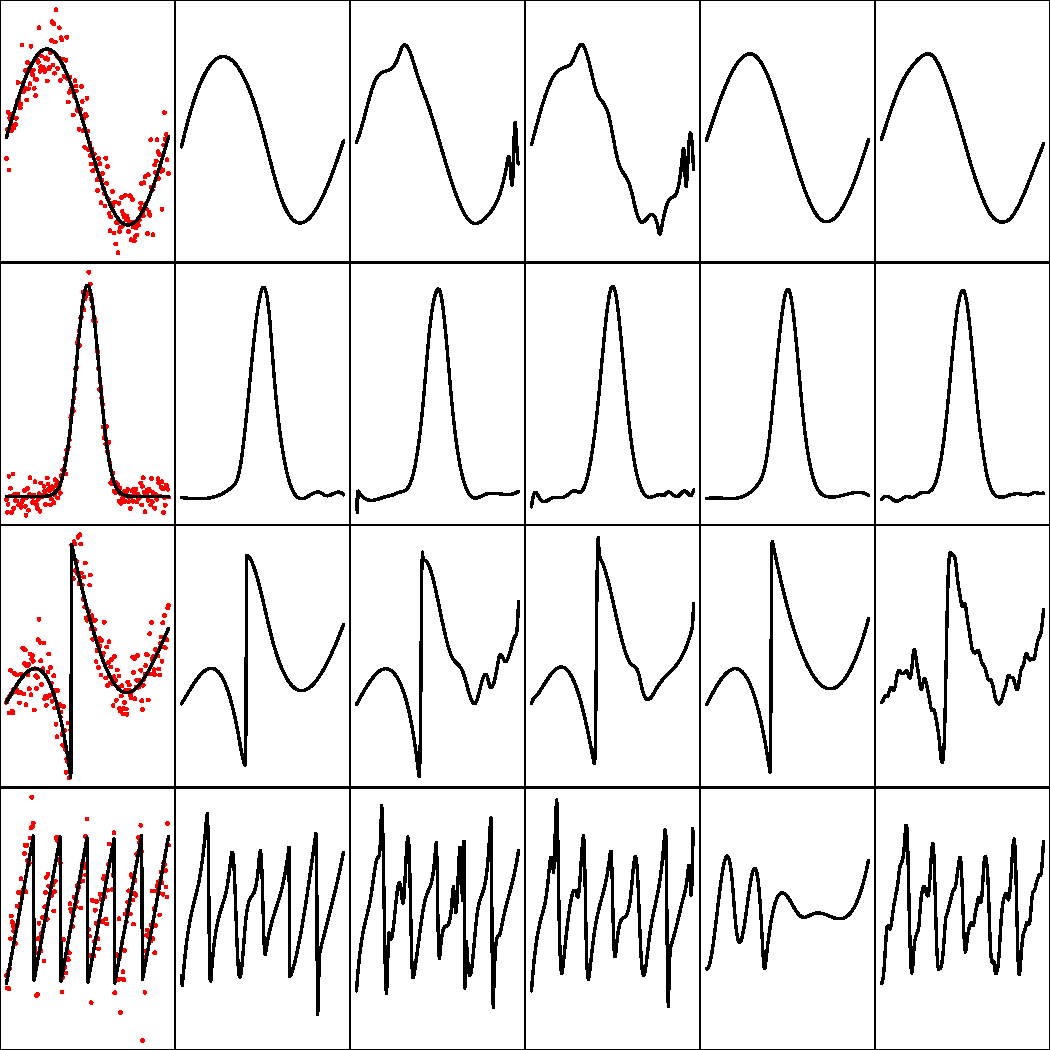
\includegraphics[width=0.85\textwidth]{Experiments/plots/curve_regression.pdf}
    \caption{Curve spline regression. It corresponds to the prediction results with $m=200$ in Cases $1.1-1.4$. From left to right, columns are respectively the ground truth with red observed points, prediction by EBARS with $\gamma=1,0.5,0$, prediction by BARS and prediction by smoothing splines.}
    \label{fig:curve}
\end{figure}

The mean squared errors are summarized in Table \ref{tab:curve}. To remove the effect of outliers, we drop out points with errors in the top or bottom $2.5\%$ to calculate censored MSE on test data. In EBARS, low $\gamma$ causes the model overfitting problem. It is clear that MSE rises up gradually as $\gamma$ decreases, especially in Case $1.3$. The behaviour is visualized in columns $2-4$ of Figure \ref{fig:curve}. This phenomenon is consistent with the theory. According to EBIC, the prior probability of the model space with $k$ knots satisfies $\pi(\mathcal{M}_k)\propto \tau(\mathcal{M}_k)^{1-\gamma}$. As $k<<n$ in practice, $\tau(\mathcal{M}_k)$ will grow with increasing number of knots. Consequently, the lower $\gamma$ means the higher $\pi(\mathcal{M}_k)$ for large $k$. Thereby more knots will be selected into the model, leading to overfitting in the end.

In this example, $\gamma=1$ gives the best performance among EBARS. Furthermore, BARS achieves similar results to EBARS $\gamma=1$ if the true knot number is relatively small, illustrated as in Cases $1.1-1.3$. However, when the required knot number is really large, BARS fails to work completely and attains a terrible MSE. See the $(4,5)$ panel of Figure \ref{fig:curve} for a graphical explanation. Besides, the smoothing spline method has a severe overfitting problem in Case $1.3$, as shown in the $(3,6)$ panel of Figure \ref{fig:curve}. This indicates that splines with many misplaced knots are inferior to adaptive knot splines in discontinuous cases.

\begin{table}
\caption{MSE on test data of five methods in Cases $1.1-1.4$}
\label{tab:curve}
\centering
\begin{tabular}{cccccccc}
\toprule
       Methods     &   $m$  & Case 1.1     & Case 1.2     & Case 1.3     & Case 1.4     \\ \midrule                               
                 
EBARS $\gamma=1$      & \multirow{5}{*}{$200$}     & 0.181(0.124) & 0.332(0.118) & 0.828(0.529) & 0.370(0.366)  \\
EBARS   $\gamma=0.5$  &       & 0.230(0.136)  & 0.389(0.184) & 1.412(0.783) & 0.368(0.150)  \\
EBARS   $\gamma=0$    &     & 0.341(0.229) & 0.464(0.201) & 1.960(0.985)  & 0.418(0.155) \\
BARS       &      & 0.178(0.150)  & 0.368(0.139) & 0.731(0.403) & 3.003(0.504) \\
SS &  & 0.137(0.088) & 0.329(0.132) & 3.772(1.687) & 0.443(0.155) \\
\midrule
EBARS $\gamma=1$     & \multirow{5}{*}{$500$}     & 0.068(0.033) & 0.147(0.061) & 0.361(0.168) & 0.079(0.033) \\
EBARS     $\gamma=0.5$   &    & 0.082(0.039) & 0.156(0.059) & 0.536(0.215) & 0.112(0.034) \\
EBARS    $\gamma=0$   &     & 0.170(0.073)  & 0.231(0.083) & 1.053(0.410)  & 0.144(0.042) \\
BARS        &     & 0.071(0.032) & 0.160(0.054)  & 0.317(0.140)  & 0.364(0.615) \\
SS & & 0.053(0.026) & 0.139(0.041) & 1.914(0.418) & 0.229(0.066) \\
\bottomrule
\end{tabular}
\end{table}